% Re-defined by Z.C.TIAN (https://github.com/doem97)
% This version comply with the Official EEE Dissertation Guidline in [EEE dissertation] (http://www.eee.ntu.edu.sg/programmes/CurrentStudents/Graduate_Coursework/mscProg/disHome/Pages/home.aspx)
% More information about dissertation can be found in [NTU thesis](http://research.ntu.edu.sg/rieo/RI/Pages/Theses--Dissertations.aspx)
% Based on W.M.ZHAO version, original link in overleaf:
% (https://www.overleaf.com/latex/templates/ntu-master-dissertation/ngnhrrwryccv)

\documentclass[12pt]{report}

%% Useful packages
\usepackage[a4paper,top=3cm,bottom=3cm,left=3.5cm,right=3cm,marginparwidth=1.75cm,headheight=22pt]{geometry}
\usepackage{amsmath}
\usepackage{cite}
\usepackage{courier}
\usepackage[export]{adjustbox}
\usepackage[nottoc,notlot,notlof]{tocbibind}
\usepackage[labelfont=bf, textfont=bf]{caption}
\usepackage{graphicx}
\usepackage{hyperref}
\usepackage{float}
\usepackage{setspace}
\usepackage{subfigure}
\usepackage{setspace}
\usepackage{lipsum}
\usepackage{fancyhdr} % Fancy header
\usepackage{url}
\usepackage{tabularx}
\usepackage[utf8]{inputenc}
\usepackage{mathptmx} %Times Font

%==== Header and Footer configure ====
% Define the plain pagestyle used by most chapters
\fancypagestyle{plain}{
\fancyhf{} % Clear header footer
\fancyhead[R]{\bf \textsl{\leftmark} \vspace{0.1in}}
\fancyfoot[R]{\thepage}
% Set the right side of the footer to be the page number
\renewcommand{\headrulewidth}{2pt}
}
% For those Chapter* (Can't use \leftmark to call their chapter name directly)
\fancypagestyle{addin}{
\fancyhf{} % Clear header footer
\fancyhead[R]{\bf \textsl{\leftmark} \vspace{0.1in}}
% Set the right side of the footer to be the page number
\fancyfoot[R]{\thepage}
\renewcommand{\headrulewidth}{2pt}
}

%==== Overall Config ====
\setlength{\parindent}{0in} % Set paragraph indent as 0
% \setlength{\fboxsep}{-0.3in}%
\setlength{\fboxrule}{0.5pt} % Set the bounding box around the image as 0.5pt
\pagestyle{plain}



\begin{document}
\fontdimen2\font=0.5em% inter word space
%==== FRONT PART====
\begin{titlepage}

\begin{figure}[h!]
\centering

\includegraphics[width=1\textwidth]{Title/NTU_logo.png}
\caption*{}
\label{fig:entropy} 
\end{figure}

\vspace{1.5in}

\centering
\Huge{\textbf{Your Title of the Dissertation\\Also Second Line}}\\[2.5in]

\LARGE{\textbf{YOUR NAME}}\\[0.5in]

\normalsize{\textbf{SCHOOL OF ELECTRICAL AND ELECTRONIC ENGINEERING}}\\[0.2in]

% \textbf{A DISSERTATION SUBMITTED IN PARTIAL FULFILMENT OF\\
% THE REQUIREMENTS FOR THE DEGREE OF\\
% MASTER OF SCIENCE IN DIGITAL MEDIA TECHNOLOGY}\\[0.25in]

\large{\textbf{2021}}
\end{titlepage}
\newpage % Coverpage
\begin{titlepage}
\begin{center}
\vspace*{2in}
\Huge{\textbf{Your Title of the Dissertation\\Also Second Line}}\\[2.5in]

\LARGE{\textbf{\MakeUppercase{YOUR NAME}}}\\[1in]

\normalsize{\textbf{\MakeUppercase{SCHOOL OF ELECTRICAL AND ELECTRONIC ENGINEERING}}}\\[0.5in]
\normalsize{\textbf{\MakeUppercase{A DISSERTATION SUBMITTED IN PARTIAL FULFILMENT OF\\THE REQUIREMENTS FOR THE DEGREE OF\\MASTER OF SCIENCE IN XXX}}}\\[0.75in]

% \textbf{A DISSERTATION SUBMITTED IN PARTIAL FULFILMENT OF\\
% THE REQUIREMENTS FOR THE DEGREE OF\\
% MASTER OF SCIENCE IN DIGITAL MEDIA TECHNOLOGY}\\[0.25in]

\large{\textbf{2021}}
\end{center}
\end{titlepage}
\newpage % Titlepage
\begin{titlepage}

\begin{center}
\Large{\bf{Statement of Originality}}
\end{center}

\vspace{0.2in}

\begin{spacing}{2}

I hereby certify that the work embodied in this thesis is the result of original research and has not been submitted for a higher degree to any other University or Institution.

\end{spacing}

\vspace{2.5cm}

\begin{center}
	\makebox[4cm]{\dotfill}  \hfill \makebox[4cm]{\dotfill}\\
	\makebox[4cm]{Date}      \hfill \makebox[4cm]{Your Name}
\end{center}
\end{titlepage}
\newpage % Titlepage
\begin{titlepage}

\begin{center}
\Large{\bf{Supervisor Declaration Statement}}
\end{center}

\vspace{0.2in}

\begin{spacing}{2}
I have reviewed the content and presentation style of this thesis and declare it is free of plagiarism and of sufficient grammatical clarity to be examined. To the best of my knowledge, the research and writing are those of the candidate except as acknowledged in the Author Attribution Statement. I confirm that the investigations were conducted in accord with the ethics policies and integrity standards of Nanyang Technological University and that the research data are presented honestly and without prejudice
\end{spacing}

\vspace{2.5cm}

\begin{center}
	\makebox[4cm]{\dotfill}  \hfill \makebox[4cm]{\dotfill}\\
	\makebox[4cm]{Date}      \hfill \makebox[4cm]{Supervisor's Name}
\end{center}
\end{titlepage}
\newpage % Titlepage
\begin{titlepage}

\begin{center}
\Large{\bf{Authorship Attribution Statement}}
\end{center}

\vspace{0.2in}

\begin{spacing}{2}

This thesis does not contain any materials from papers published in peer-reviewed journals or from papers accepted at conferences in which I am listed as an author.

\end{spacing}

\vspace{2.5cm}

\begin{center}
	\makebox[4cm]{\dotfill}  \hfill \makebox[4cm]{\dotfill}\\
	\makebox[4cm]{Date}      \hfill \makebox[4cm]{Your Name}
\end{center}
\end{titlepage}
\newpage % Titlepage

%\begingroup
%\let\cleardoublepage\clearpage

\pagenumbering{roman}

\renewcommand*\contentsname{\centering Table of Contents}
\tableofcontents
\newpage

%=== FRONT PART ===
%=== ABSTRCT ===
\newpage

\chapter*{\centering Abstract}
\markboth{Abstract}{}
% \vspace{-0.3in}

\begin{spacing}{1.5}
\setlength{\parskip}{0.3in}

\addcontentsline{toc}{chapter}{Abstract}

Put your abstracts here. The Abstract should be a short and concise passage on the important work and contributions of the project: the motivation and the problem pursued, the method you employed and the results obtained, highlighting the significant achievements. It should not contain peripheral things like summary of literature review, and it is not good enough to say that a certain issue has been studied without stating the results of the study. Generally, one page is about the right length for the Abstract.

\par
\textbf{Keywords:} Dissertation, keywords.
\end{spacing}
\newpage
%=== END OF ABSTRACT ===

%=== FRONT PART ===
%=== ACKNOWLEDGEMENT ===
\fancypagestyle{addin}{
\fancyhead[R]{\bf \textsl{ACKNOWLEDGEMENTS} \vspace{0.1in}}
}
%\begin{center}
\chapter*{\centering Acknowledgements}
\begin{spacing}{1.5}
\setlength{\parskip}{0.3in}
\thispagestyle{addin}
%\end{center}
\addcontentsline{toc}{chapter}{Acknowledgement}

Acknowledgements goes here.

\end{spacing}
\newpage
%=== END OF ACKNOWLEDGEMENT  ===

%=== FRONT PART ===
%=== ACRONYMS ===
\fancypagestyle{addin}{
\fancyhead[R]{\bf \textsl{ACRONYMS} \vspace{0.1in}}
}
%\begin{center}
\chapter*{\centering Acronyms}
\begin{spacing}{1.5}
\setlength{\parskip}{0.3in}
\thispagestyle{addin}
%\end{center}
\addcontentsline{toc}{chapter}{Acronyms}

Acronyms goes here.
\end{spacing}
\newpage
%=== END OF ACRONYMS ===

%=== FRONT PART ===
%=== SYMBOLS ===
\fancypagestyle{addin}{
\fancyhead[R]{\bf \textsl{SYMBOLS} \vspace{0.1in}}
}
%\begin{center}
\chapter*{\centering Symbols}
\begin{spacing}{1.5}
\setlength{\parskip}{0.3in}
\thispagestyle{addin}
%\end{center}
\addcontentsline{toc}{chapter}{Symbols}

Symbols goes here.
\end{spacing}
\newpage
%=== END OF ACKNOWLEDGEMENT  ===



\renewcommand{\listfigurename}{\centering List of Figures}
\listoffigures
\addcontentsline{toc}{chapter}{Lists of Figures}
\newpage

\renewcommand{\listtablename}{\centering List of Tables}
\listoftables 
\addcontentsline{toc}{chapter}{Lists of Tables}
\newpage

%\endgroup

%==== MAIN PART ====

\pagenumbering{arabic}
%=== CHAPTER ONE (1) ===
%=== INTRODUCTION ===

\chapter{Introduction}
\begin{spacing}{1.5}
\setlength{\parskip}{0.3in}

The first chapter of the dissertation is almost invariably the Introduction. Generally, its purpose is to lead the readers into the problem you intend to attack in the project, to set the scene. The main points here consist of the background to the problem and your motivation in solving it. This then leads into the objectives and the scope of the project. It is good to conclude your Introduction with a section on the layout of the dissertation. It prepares the readers for what is to come

\section{Background}


Background goes here. Also you can put in some references~\cite{ronneberger2015unet}.

Here is a sample of table in \autoref{tabelsample}

\begin{table}[ht]
\centering
\caption{A table without vertical lines.}
\label{tabelsample}
\begin{tabular}[t]{lcc}
\hline
&Treatment A&Treatment B\\
\hline
John Smith&1&2\\
Jane Doe&--&3\\
Mary Johnson&4&5\\
\hline
\end{tabular}
\end{table}%

Also can try to refer to this image in \autoref{fig:boundingboxexample}.


\begin{figure}[ht]
\centering
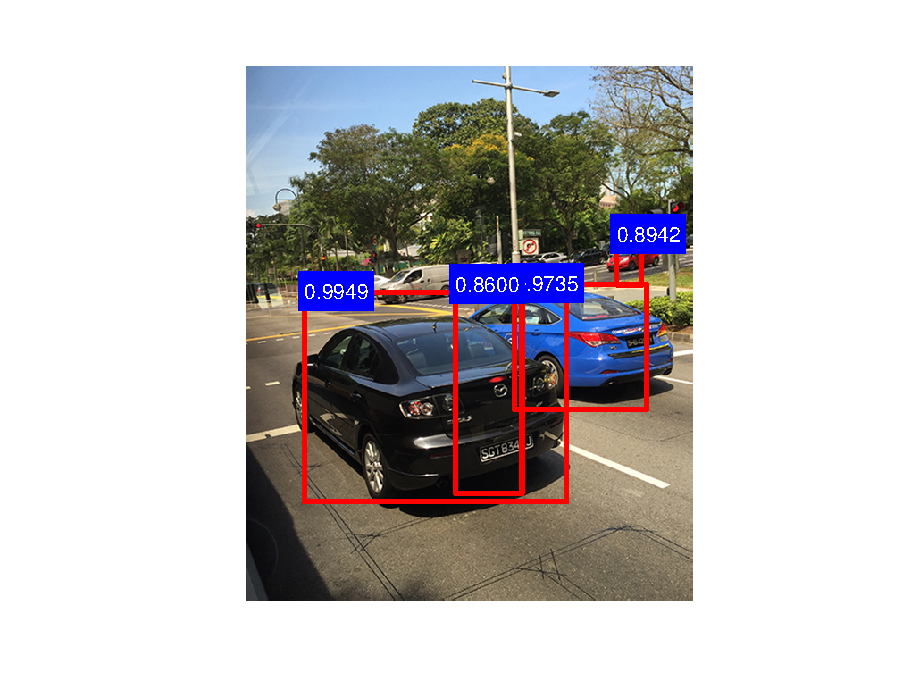
\includegraphics[width=4in, fbox]{Chapter1/boundingbox.eps}
\caption{Bounding-box example of cars.}
\label{fig:boundingboxexample} 
\end{figure}


\section{Motivation}


\section{Objectives and Specifications}



\section{Major contribution of the Dissertation}



\section{Organisation of the Dissertation}


\end{spacing}
%=== END OF CHAPTER ONE ===
\newpage



%=== CHAPTER TWO (2) ===
%=== Literature Review ===

\chapter{Literature Review}
\begin{spacing}{1.5}
\setlength{\parskip}{0.3in}

\section{Overview}

Then comes the main part of your work. To lay the ground, there should first be a chapter on what has been done before on the problem - a Literature Review. This is an important section because it shows that you do not narrowly focus only on what you do, but are aware of the
related work elsewhere, some of which might be instructive to your solving the problem. It can also explain why you are taking the direction you do.

\section{One}
(Co-localization methods of auto-drawing bbox)

\section{Two}
(Propagate bbox by co-segmentation)

\section{Three}
(Suggesting images to users)


%=== END OF CHAPTER TWO ===
\end{spacing}
\newpage

%=== CHAPTER THREE (3) ===
%=== (Actual work done and contribution, including literature survey) ===

\chapter{Approach}
\begin{spacing}{1.5}
\setlength{\parskip}{0.3in}
%  (Actual work done and contribution, including literature survey)


\section{One}

The next few chapters should describe the work you have done in tackling the problem. There might be a chapter on the fundamental theories relevant to the solution you are pursuing, or the supporting technologies you need in implementing the solution. Then there should be a chapter on the solution itself, followed by a chapter on the results and analysis of the results

\section{Two}


\section{Three}


%=== END OF CHAPTER THREE ===
\end{spacing}
\newpage

%=== CHAPTER FOUR (4) ===
%=== Test and Experiments ===

\chapter{Test and Experiments}
\begin{spacing}{1.5}
\setlength{\parskip}{0.3in}

\section{One}


\section{Two}

\section{Three}


%=== END OF CHAPTER FOUR ===
\end{spacing}
\newpage

%=== CHAPTER FIVE (5) ===
%=== Discussion ===

\chapter{Discussion}
\begin{spacing}{1.5}
\setlength{\parskip}{0.3in}

\section{One}

Generally, there should be no more than six or seven chapters in your dissertation. If you have more than that, you should take a close look at its orgainsation and see if certain chapters can be merged.

\section{Two}

\section{Three}


%=== END OF CHAPTER FIVE ===
\end{spacing}
\newpage

%=== CHAPTER SIX (6) ===
%=== Conclusion and Recommendations ===

\chapter{Conclusion and Recommendations}
\begin{spacing}{1.5}
\setlength{\parskip}{0.3in}

\section{One}

The last chapter is always the Conclusion. This generally should have three parts. The first is a concise summary of the work you have done. In a way, this is similar to the abstract. Then there is the conclusion, in which you highlight the significance of the results, and perhaps the consequences of the results, critically where necessary. The last thing is usually recommendations and/or future work, in which you identify the inadequacies of what you have done, and suggest how the gaps may be plugged.

\section{Two}

Documents that are prepared with the help of other sources should have a list of sources cited. A list of References contains only sources the writer quotes directly, takes original ideas from, and refers to in the dissertation should be included. In reports where the subject is primarily scientific, the list of references is the most widely accepted way to cite specific sources.

\section{Three}

\section{Four}

\subsection{Six}


%=== END OF CHAPTER SIX ===
\end{spacing}
\newpage

%==== ENDING PART ===

\renewcommand\bibname{References}
\bibliographystyle{unsrt}
\begin{spacing}{1.5}
\bibliography{Ref/References}
\end{spacing}
\newpage

%=== APPENDIX ===
%=== APPENDIX ===
\chapter*{Appendix A}
\fancypagestyle{addin}{
\fancyhead[R]{\textsl{APPENDIX A} \vspace{0.1in}}
}
\thispagestyle{addin}
\addcontentsline{toc}{chapter}{Appendix A}
\setlength{\parskip}{0.3in}
\begin{spacing}{1.5}
(Code Here)

The Appendix contains related data not necessary to the immediate understanding of the discussion in the report. This may contain materials such as: tables, graphs, illustrations, description of equipment, samples of forms, data sheets, questionnaires, equations, and any material that must be included for record purposes.
Each entry (sample forms, detailed data for references, tables, pictures, questionnaires, charts, maps, graphic representations) in the appendix requires an identifying title. Every entry in the appendix must be referred to in the body of the report. Each appendix must be lettered, beginning with Appendix A. The list of appendices should be appearing in the table of contents following the list of references entry.

\end{spacing}
\newpage

\chapter*{Appendix B}
\fancypagestyle{addin}{
\fancyhead[R]{\textsl{APPENDIX B} \vspace{0.1in}}
}
\thispagestyle{addin}
\addcontentsline{toc}{chapter}{Appendix B}
\begin{spacing}{1.5}

(Code Here)

Usually codes lah.

\end{spacing}
%=== END OF CHAPTER SIX ===
\newpage

%==== END OF ALL ===
\end{document}
